\documentclass[dvipdfmx,a4paper,11pt]{jsarticle}


% 数式
\usepackage{amsmath,amsfonts}
\usepackage{bm}
\usepackage{amsthm}
\usepackage{amssymb}
\usepackage{tcolorbox}
% 画像
% \usepackage[dvipdfmx]{graphicx,color}

\usepackage[%
dvipdfmx, %欧文ではコメントアウトする
setpagesize=false,
bookmarks=true,
bookmarksdepth=tocdepth,
bookmarksnumbered=true,
colorlinks=true,
linkcolor=blue,
citecolor=blue,
urlcolor=blue,
pdftitle={},
pdfsubject={},
pdfauthor={},
pdfkeywords={}
]{hyperref}

\usepackage{pxjahyper}
\usepackage{tikz}
\usetikzlibrary{intersections,calc,arrows.meta}


\begin{document}
\theoremstyle{plain}
\newtheorem{thm}{Theorem}[section]
\newtheorem{lem}[thm]{Lemma}
\newtheorem{prop}[thm]{Proposition}
\newtheorem{cor}[thm]{Corollary}
\newtheorem{conj}[thm]{Conjecture}

\theoremstyle{definition}
\newtheorem{ass}[thm]{Assumption}
\newtheorem{dfn}[thm]{Definition}

\theoremstyle{remark}
\newtheorem{rem}[thm]{Remark}

\theoremstyle{plain}
\newtheorem*{thm*}{Theorem}
\newtheorem*{lem*}{Lemma}
\newtheorem*{prop*}{Proposition}
\newtheorem*{cor*}{Corollary}
\newtheorem*{conj*}{Conjecture}

\theoremstyle{definition}
\newtheorem*{ass*}{Assumption}
\newtheorem*{dfn*}{Definition}

\theoremstyle{remark}
\newtheorem*{Proof}{Proof}

\numberwithin{equation}{section}

\theoremstyle{remark}
\newtheorem*{rem*}{Remark}

\title{位相幾何}
\date{}
\author{Fefr}
\maketitle
\tableofcontents
\clearpage

%--------------------本文--------------------%

\section{位相空間の(コ)ホモロジー}

\subsection{圏と関手}

圏の定義は略。\\
圏の例をすこしあげる。
\begin{tcolorbox}[title = 例1]
  位相空間$X$から位相空間$Y$への写像の族$f_{i}:X\to Y$に対し、写像$F:X\times [0,1] \to Y$を
  \begin{equation*}
    F(x,t)=f_{i}(x)\qquad (x\in X,t \in [0,1])
  \end{equation*}
  で定義するとき、$F$が連続ならば写像族$\{f_i\}$を$f_0$から$f_1$への\textgt{ホモトピー}(homotopy)という。\\
  連続写像$f,f':X\to Y$に対し、$f$から$f'$へのホモトピーが存在するとき$f$は$f'$に\textgt{ホモトープ}(homotop)
  であるといい、$f\simeq f':X\to Y$で表す。\\
  ホモトープという関係は同値関係となる。\\
  実際、反射律は$f\simeq f:X\to Y$は$f_{t}=f$とすることにより、対称律は$f\simeq f':X\to Y$とすると、
  $f'$の$f$へのホモトピー$\{f'_{t}\}$は$f$の$f'$へのホモトピー$\{f_{t}\}$を用いて$f'_{t}=f_{1-t}$で与えられる。
  推移律は、$f\simeq f',f'\simeq f'':X\to Y$ならば$f$の$f''$へのホモトピー$\{h_{t}\}$が
  $f$から$f'$へのホモトピー$\{f_{t}\}$、$f'$から$f''$へのホモトピー$\{g_{t}\}$を用いて
  \begin{equation*}
    h_{t}=\left\{ 
    \begin{alignedat}{2}   
      &f_{2t}  \quad &(0\leq t\leq 1/2)\\   
      &g_{2t-1}\quad &(1/2\leq t\leq 1)
    \end{alignedat} 
    \right.
  \end{equation*}
  で与えられる。\\
  上の同値類を連続写像の\textgt{ホモトピー類}(えいやくだれか教えて)という。\\
  明らかに$f\simeq f':X\to Y$で$g\simeq g':Y\to Z$ならば\\
  \begin{equation*}
    g\circ f\simeq g\circ f'\simeq g'\circ f'\simeq g'\circ f:X \to Z
  \end{equation*}
  である。($\{g\circ f_{t}\}$が$g\circ f$から$g\circ f'$へのホモトピーを与え、$\{g_{t}\circ f'\}$が$g\circ f'$から$g'\circ f'$へのホモトピーを与える。)\\
  すなわち、ホモトープな連続写像の合成はホモトープである。\\
  よって、対象を位相空間とし、射を連続者像のホモトピー類で定義することにより、1つの圏が得られる。
\end{tcolorbox}

\clearpage

加群,加群の準同型写像の定義は略。$R$加群、$R$準同型写像を単に加群、準同型写像という。
簡単のため$R$を可換環と仮定する。可換性が必要がない場面もある。
\begin{tcolorbox}[title = 例2]
  整数の集合$\mathbf{Z}$を添字集合とする$R$上の加群の族$C=\{C_{q}\}$を$R$上の\textgt{次数つき加群}(graded module)
  といい、$C_{q}$の元$c$を$C$の\textgt{次数$q$の元}といって、$q=\text{deg}\ c$と書く。$C,C'$を次数つき加群とし、
  $d$を1つの整数とする。このとき$\mathbf{Z}$を添字集合とする準同型写像$\varphi_{q}:C_{q} \to C_{q+d}$の族$\varphi = \{\varphi_{q}\}$を
  $C$から$C'$への\textgt{次数$d$の準同型写像}といい、$\varphi : C\to C'$で表す。\\
  $C''$も加群とし、$\varphi' : C'\to C''$を次数$d'$の準同型写像とするとき、次数$d+d'$の準同型写像$\varphi' \circ \varphi : C\to C''$を
  \begin{equation*}
    (\varphi' \circ \varphi)_{q} = \varphi'_{d+q} \circ \varphi_{q}
  \end{equation*} 
  で定義し、$\varphi$と$\varphi'$の合成という。
  いま、次の二つの圏が得られる。
  \begin{itemize}
    \item 次数つき加群を対象とし、任意の次数の準同型写像を射とする圏
    \item 次数つき加群を対象とし、次数$0$の準同型写像を射とする圏
  \end{itemize}
\end{tcolorbox}

\begin{tcolorbox}[title = 例3]
  $R$上の次数つき加群$C$において、次数$-1$の準同型写像$\partial : C\to C$で
  \begin{equation*}
    \partial \circ \partial = 0
  \end{equation*}
  を満たすものが与えられたとき、$(C,\partial)$を\textgt{$R$上のチェイン複体}(chain complex)という。
  チェイン複体は加群$C_{q}$と準同型写像$\partial_{q}:C_{q}\to C_{q-1}$の列
  \begin{center}
    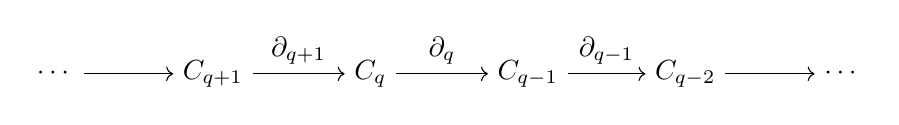
\begin{tikzpicture}[auto]
      \node (a) at (0, 1.2) {$\cdots$}; \node (b) at (2.0, 1.2) {$C_{q+1}$};
      \node (c) at (4.0, 1.2) {$C_{q}$}; \node (d) at (6.0, 1.2) {$C_{q-1}$};
      \node (e) at (8.0, 1.2) {$C_{q-2}$}; \node (f) at (10.0, 1.2) {$\cdots$};
      
      \draw[->] (a) to node {} (b); \draw[->] (b) to node {$\partial_{q+1}$} (c);
      \draw[->] (c) to node {$\partial_{q}$} (d); \draw[->] (d) to node {$\partial_{q-1}$} (e);
      \draw[->] (e) to node {} (f);
    \end{tikzpicture}
  \end{center}
  で、各$q$に対し
  \begin{equation*}
    \partial_{q-1} \circ \partial_{q} = 0
  \end{equation*}
  の成り立つもの、と言い換えることができる。$\partial = \{\partial_{q}\}$を\textgt{バウンダリ作用素}(えいやくd(((()という。
  チェイン複体$(C,\partial)$を単に$C$で表す。\\
  $C,C'$をチェイン複体とするとき、次数$0$の準同型写像$\varphi : C\to C'$で、$C,C'$のバウンダリ作用素$\partial$に対し
  \begin{equation*}
    \partial \circ \varphi = \varphi \circ \partial
  \end{equation*}
  を満たすものを\textgt{チェイン写像}(chain map)という。すなわち、準同型写像$\varphi_{q} : C_{q} \to C'_{q}$の族
  $\varphi = \{\varphi_{q}\}$で、各$q$に対し
  \begin{equation*}
    \partial_{q} \circ \varphi_{q} = \varphi_{q-1} \circ \partial_{q}
  \end{equation*}
  の成り立つものがチェイン写像である。\\
  チェイン複体の恒等写像(恒等射)はチェイン写像であり($\partial\varphi = \varphi\partial$で次数$0$だから)\\
  チェイン写像の合成はチェイン写像である。(確かめること)\\
  よって、チェイン複体を対象とし、射をチェイン写像とすることにより、1つの圏を得る。
\end{tcolorbox}

\begin{tcolorbox}[title = 例4]
  チェイン写像$\varphi,\varphi':C\to C'$に対し、次数$+1$の準同型写像$\Phi : C\to C'$があって、
  \begin{equation*}
    \partial \circ \Phi + \Phi \circ \partial = \varphi - \varphi'
  \end{equation*}
  が成り立つとき、$\varphi$は$\varphi'$への\textgt{チェインホモトープ}であるといい、$\varphi \simeq \varphi' : C\to C'$で表す。
  $\Phi$を$\varphi$の$\varphi'$への\textgt{チェインホモトピー}という。
\end{tcolorbox}



\end{document}
